\documentclass[12pt, a4paper]{article}
    
\usepackage{homework}
\usepackage{amsmath}				% For Math
\usepackage{fancyhdr}				% For fancy header/footer
\usepackage{graphicx}				% For including figure/image
\usepackage{cancel}					% To use the slash to cancel out stuff in work
\usepackage{multirow}

%%%%%%%%%%%%%%%%%%%%%%
% Set up fancy header/footer
\pagestyle{fancy}
\setlength{\headheight}{30pt}
\fancyhead[LO,L]{Name: Yu Ching Hei\\SID: 1155193237\\email: chyu2@cse.cuhk.edu.hk}
\fancyhead[CO,C]{}
\fancyhead[RO,R]{CENG3420 Computer Organization and Design\\Homework 2\\Date: \today}
\fancyfoot[LO,L]{}
\fancyfoot[CO,C]{}
\fancyfoot[RO,R]{Page \thepage}
\renewcommand{\headrulewidth}{0.4pt}
\renewcommand{\footrulewidth}{0.4pt}
%%%%%%%%%%%%%%%%%%%%%%

\begin{document}
\noindent What is your last digit of your SID (0 is regarded as 10)? This value is defined as
NUM\_1 in the whole question paper. (Since my last digit is 7, NUM\_1 is 7)\\

\begin{q}{15}
Consider the following RISC-V instructions. Please note that we treat 
NUM\_1\%2 and NUM\_1\%2+1 as decimal values.
\begin{code}
    li a1, NUM_1%2
    li a2, NUM_1%2+1
    li a3, 6
    LOOP:
    slti t0, a3, 1
    bne t0, zero, DONE
    add a4, a1, a2
    addi a1, a2, 0
    addi a2, a4, 0
    addi a3, a3, -1
    jal x0, LOOP
    DONE:
    # end of the program
\end{code}
\begin{enumerate}
    \item How many times is the branch instruction executed? (7\%)
    \item What are the final values of a1 and a2. (8\%)
\end{enumerate}
\end{q}

\begin{ans}
    \begin{enumerate}
        \item 6 times (with one more check which is line 5 and 6 as shown)
        \item a1 = 21, a2 = 34
    \end{enumerate}
\end{ans}
\pagebreak
\begin{q}{20}
Read through the multiplication / devision algorithm: 
\begin{center}
    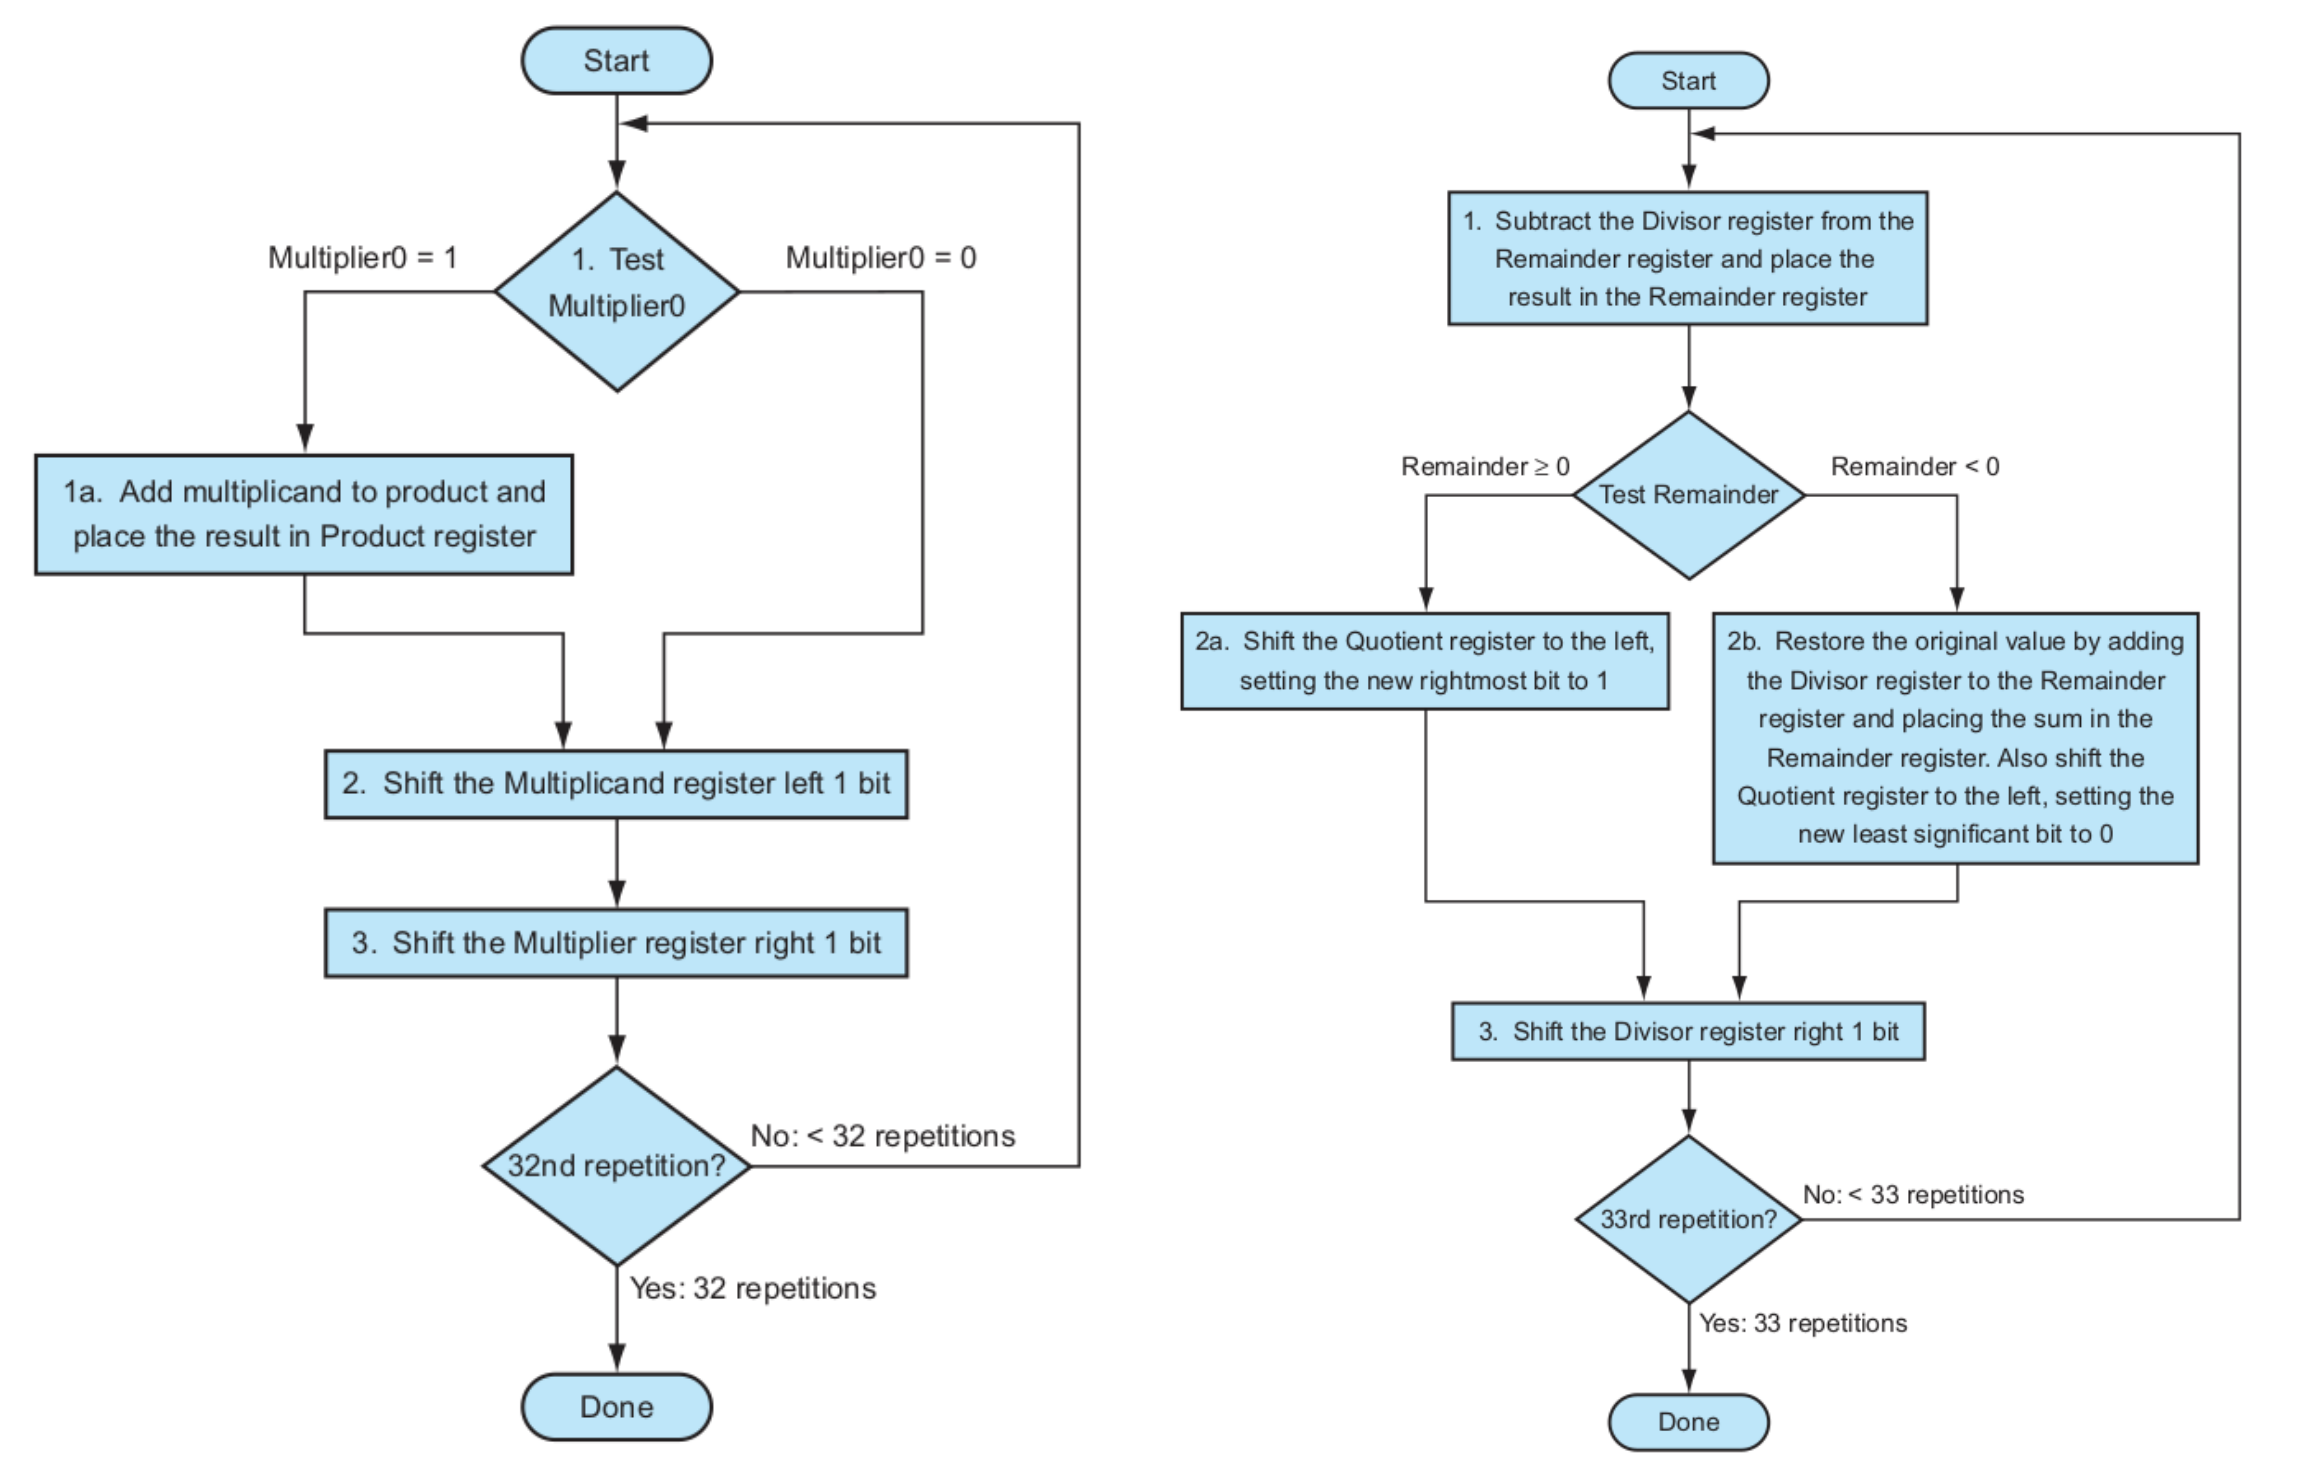
\includegraphics[scale=0.36]{q2.png}
    Left: multiplication algorithm, Right: division algorithm
\end{center}
Write down the step by step procedure to calculate 5×2 or 0101×0010. Use Multiplier0
to indicate the least significant bit of the multiplier. List the initial values and the values
in 1st to 4th iterations of Multiplier, Multiplier0, Multiplicand and Product. In each
iteration, list the values after 1, 2 and 3 steps in Figure 1 left separately. (Represent
Multiplier as 4bits, Multiplier0 as 1bit, Multiplicand as 8bits, Product as 8bits.)
\end{q}
\begin{ans}
    \begin{center}
        \begin{tabular}{|c|c|c|c|c|c|}
            \hline
            Iteration & Step & Multiplier & Multiplier0 & Mcand & Product\\
            \hline
            0 & Initial value & 010\underline{1} & 1 & 0000 0010 & 0000 0000\\
            \hline
            \multirow{3}{*}{1} & \multicolumn{1}{|c}{1$\Rightarrow$Prod=Prod+Mcand} & \multicolumn{1}{|c}{0101} & \multicolumn{1}{|c}{1} & \multicolumn{1}{|c}{0000 0010} & \multicolumn{1}{|c|}{0000 0010} \\\cline{2-6}
                                & \multicolumn{1}{|c}{Shift left Multiplicand} & \multicolumn{1}{|c}{0101} & \multicolumn{1}{|c}{1} & \multicolumn{1}{|c}{0000 0100} & \multicolumn{1}{|c|}{0000 0010} \\\cline{2-6}
                                & \multicolumn{1}{|c}{Shift right Multiplier} & \multicolumn{1}{|c}{001\underline{0}} & \multicolumn{1}{|c}{0} & \multicolumn{1}{|c}{0000 0100} & \multicolumn{1}{|c|}{0000 0010} \\\hline

            \multirow{2}{*}{2} 
                                & \multicolumn{1}{|c}{Shift left Multiplicand} & \multicolumn{1}{|c}{0010} & \multicolumn{1}{|c}{0} & \multicolumn{1}{|c}{0000 1000} & \multicolumn{1}{|c|}{0000 0010} \\\cline{2-6}
                                & \multicolumn{1}{|c}{Shift right Multiplier} & \multicolumn{1}{|c}{000\underline{1}} & \multicolumn{1}{|c}{1} & \multicolumn{1}{|c}{0000 1000} & \multicolumn{1}{|c|}{0000 0010} \\\hline

            \multirow{3}{*}{3} & \multicolumn{1}{|c}{1$\Rightarrow$Prod=Prod+Mcand} & \multicolumn{1}{|c}{0001} & \multicolumn{1}{|c}{1} & \multicolumn{1}{|c}{0000 1000} & \multicolumn{1}{|c|}{0000 1010} \\\cline{2-6}
                                & \multicolumn{1}{|c}{Shift left Multiplicand} & \multicolumn{1}{|c}{0001} & \multicolumn{1}{|c}{1} & \multicolumn{1}{|c}{0001 0000} & \multicolumn{1}{|c|}{0000 1010} \\\cline{2-6}
                                & \multicolumn{1}{|c}{Shift right Multiplier} & \multicolumn{1}{|c}{000\underline{0}} & \multicolumn{1}{|c}{0} & \multicolumn{1}{|c}{0001 0000} & \multicolumn{1}{|c|}{0000 1010} \\\hline

            \multirow{2}{*}{4}
                                & \multicolumn{1}{|c}{Shift left Multiplicand} & \multicolumn{1}{|c}{000\underline{0}} & \multicolumn{1}{|c}{0} & \multicolumn{1}{|c}{0010 0000} & \multicolumn{1}{|c|}{0000 1010} \\\cline{2-6}
                                & \multicolumn{1}{|c}{Shift right Multiplier} & \multicolumn{1}{|c}{000\underline{0}} & \multicolumn{1}{|c}{0} & \multicolumn{1}{|c}{0010 0000} & \multicolumn{1}{|c|}{0000 1010} \\\hline
        \end{tabular}
    \end{center}
\end{ans}
\pagebreak

\begin{q}{20}
    IEEE 754 Floating-Point Standard
    \begin{enumerate}
        \item What decimal number does this single precision float $\mathtt{C13C0000_{16}}$ represent? (Show your work.) (10 \%)
        \item What is -1.510 in IEEE single precision binary floating point format? (Show your work.) (10\%)
    \end{enumerate}
\end{q}
\begin{ans}
    \begin{enumerate}
        \item \begin{enumerate}
                \item by breaking the hexadecimal number into binary, we get $$\mathtt{C13C0000_{16}}=\mathtt{1100 0001 0011 1100 0000 0000 0000 0000_2}$$
                \item the first bit indicate the sign, in this case it is a negative number
                \item the next 8 bits are used to express the exponent offset by -127, so the exponent in this case is $\mathtt{10000010_2 - 127_{10} = 130_{10} - 127_{10} = 3_{10}}$ 
                \item the following 23 bits are the mantissa
            \end{enumerate}
    \end{enumerate}
\end{ans}
\end{document}
